% point_encadrant.tex
% =====================================================================
% Point d'avancement avec Raphael Minato -- support de reunion de travail.
%
% EN FRANCAIS, contrairement au pitch et au rapport : c'est du meta au
% sens de `.claude/rules/depot.md`, pas un livrable. Les livrables
% (rapport, poster, soutenance) restent en anglais.
%
% PARTI PRIS
%   Douze slides, dont trois qui posent une QUESTION a l'encadrant plutot
%   qu'un resultat. L'objet de la reunion est ce qu'on ne peut pas
%   trancher seuls : la portee de notre resultat sur lambda, la fenetre
%   de A, et le perimetre. Le reste sert a y amener.
%   Un fil d'Ariane recentre a chaque slide de question.
%
% SCHEMAS
%   Les quatre schemas TikZ sont dans `point_encadrant_schemas.tex` :
%   ils sont STYLISES, SANS DONNEES, et le fichier est separe pour que
%   leurs coordonnees n'entrent pas dans le controle de tracabilite.
%
% TRACABILITE DES CHIFFRES -- chaque valeur de ce fichier, et sa source
%   slide 4  P_miss 0.0905 / 0.9715 / 1.0000 + Wilson ... rapport_final.tex tab:race
%            borne de Frechet 0.91 a Delta_e = 0.028 ..... rapport_final.tex tab:frechet
%   slide 5  M_crit = 0 a Delta_e = 0.33, F = 0.49 ....... rapport_final.tex l. 458-461
%   slide 6  0 violation sur 5 795 comparaisons .......... rapport_final.tex l. 523
%            6.0 a 14.3 fois plus tard .................... rapport_final.tex l. 533
%            facteur 1.8 contre 5.8 attendus .............. rapport_final.tex, encadre budget
%            rectangle : +23 a +43 % sous 0.19,
%            -6.9 a -41.1 % au-dessus ..................... rapport_final.tex l. 694-696
%   slide 7  tau_b(tau_ARF, A(H))   +0.0526, 0/18 ........ QCD_correlations_stratifiees_full
%            tau_b(tau_ARF, S_max)  +0.2129, 15/18 ....... idem
%   slide 8  detection / victoire / fausses alarmes ...... QE_balayage_lambda_n2000.parquet
%            (colonnes taux_detection, taux_victoire,
%             taux_fausse_alarme, fa_k, fa_lo, fa_hi)
%   slide 9  0 % de victoires a Delta_e = 0.028 .......... QE_balayage_lambda_par_amplitude_n2000
%            resolution du temoin 0.19 % a n = 2 000 ..... balayage_lambda.py, en-tete
%   slide 10 A(H) negative des Delta_e = 0.482, -20.8 .... rapport_final.tex l. 700-701
%            erreur sous son socle 1 934 pas sur 2 000 ... rapport_final.tex l. 700
%
% CONTROLE
%   cd ../04_experimentations/resultats_R2/scripts
%   PYTHONHASHSEED=0 python verif_chiffres_tex.py ../../../05_presentation/point_encadrant.tex
%
% COMPILATION
%   lualatex point_encadrant.tex   (deux passes, positions TikZ)
% =====================================================================

\documentclass[aspectratio=169,11pt]{beamer}

\usetheme{Madrid}
% Meme reglage que le pitch : sous Madrid en 16:9 la marge par defaut
% n'est que de 3,9 mm, et tout semble deborder en plein ecran.
\setbeamersize{text margin left=1cm, text margin right=1cm}
\usepackage[french]{babel}
\usepackage{amsmath,amssymb}
\usepackage{graphicx}
\usepackage{booktabs}
\usepackage{tikz}
% siunitx : la SOURCE porte le point decimal, pour que
% `verif_chiffres_tex.py` puisse controler chaque valeur ; l'affichage
% porte la virgule et l'espace fine des milliers. Ecrire 0{,}0905 en
% clair rendrait le chiffre invisible au controle de tracabilite.
\usepackage{siunitx}
% group-digits=integer : sans lui, 0.1039 s'affiche « 0,103 9 » -- siunitx
% groupe aussi la partie decimale par defaut.
\sisetup{output-decimal-marker={,}, group-separator={\,},
         group-minimum-digits=4, group-digits=integer, detect-all}
\setbeamertemplate{navigation symbols}{}
\graphicspath{{../04_experimentations/resultats_R2/resultats/figures/slides_latex/}{../04_experimentations/resultats_R2/resultats/figures/}}

% point_encadrant_schemas.tex
% =====================================================================
% Les schemas TikZ de `point_encadrant.tex`, et le fil d'Ariane.
%
% POURQUOI UN FICHIER SEPARE
%   `verif_chiffres_tex.py` extrait tout litteral numerique du .tex et le
%   cherche dans les Parquet. Les coordonnees TikZ en seraient ramassees
%   comme des mesures introuvables. Les schemas vivent donc ici, et le
%   controle de tracabilite porte sur `point_encadrant.tex` seul -- ou
%   chaque chiffre est bien une mesure.
%
%   Corollaire : AUCUN chiffre de mesure ne doit entrer dans ce fichier.
%   Les quatre schemas sont STYLISES, SANS DONNEES, comme les trois
%   schemas du pitch, et chaque legende le dit a l'ecran.
% =====================================================================

\usetikzlibrary{positioning, arrows.meta, patterns, decorations.pathreplacing}

% --- Palette : lisible en N&B comme le veut la regle de redaction ------
\definecolor{ctranche}{gray}{0.28}
\definecolor{couvert}{gray}{0.62}
\definecolor{cfond}{gray}{0.93}

% ---------------------------------------------------------------------
% Fil d'Ariane : les cinq pastilles, celle en cours en gras.
% L'argument est le RANG de la pastille active (1 = A ... 5 = lambda),
% pas son nom : comparer des chaines demanderait \pdfstrcmp, dont le nom
% n'est pas stable entre pdftex et luatex.
% Usage : \fildariane{3}   % met C en gras
% ---------------------------------------------------------------------
\newcommand{\fildariane}[1]{%
  \begin{tikzpicture}[baseline=-2pt]
    \foreach \q [count=\i] in {A,B,C,D,{$\lambda$}} {
      \pgfmathsetmacro{\x}{(\i-1)*1.0}
      \ifnum\i=#1
        \node[draw=ctranche, fill=ctranche, text=white, rounded corners=2pt,
              minimum width=0.72cm, minimum height=0.30cm,
              font=\bfseries\scriptsize] at (\x,0) {\q};
      \else
        \node[draw=couvert, text=couvert, rounded corners=2pt,
              minimum width=0.72cm, minimum height=0.30cm,
              font=\scriptsize] at (\x,0) {\q};
      \fi
    }
  \end{tikzpicture}%
}

% ---------------------------------------------------------------------
% Schema 1 -- la carte des questions (slide 2)
% ---------------------------------------------------------------------
\newcommand{\schemaCarte}{%
\begin{tikzpicture}[
    q/.style={draw=ctranche, fill=cfond, rounded corners=3pt,
              text width=2.15cm, minimum height=1.55cm, align=center,
              font=\scriptsize, inner sep=3pt},
    ouvert/.style={q, draw=couvert, dashed, fill=white},
    lien/.style={-{Stealth[length=4pt]}, couvert, thick}]

  \node[q] (a) at (0,0)
    {\textbf{A}\\[1pt]\scriptsize la course\\[2pt]\tiny tranchée};
  \node[q] (b) at (2.6,0)
    {\textbf{B}\\[1pt]\scriptsize l'indépendance\\[2pt]\tiny tranchée};
  \node[q] (c) at (5.2,0)
    {\textbf{C}\\[1pt]\scriptsize le chronomètre\\[2pt]\tiny tranchée};
  \node[q] (d) at (7.8,0)
    {\textbf{D}\\[1pt]\scriptsize l'instrumentation\\[2pt]\tiny tranchée};
  \node[ouvert] (l) at (10.4,0)
    {$\boldsymbol\lambda$\\[1pt]\scriptsize le réglage\\[2pt]\tiny \textbf{à confirmer}};

  \draw[lien] (a) -- (b);
  \draw[lien] (b) -- (c);
  \draw[lien] (c) -- (d);
  \draw[lien, ctranche] (d) -- (l);

  \node[couvert, font=\tiny, below=1pt of a] {théorique};
  \node[couvert, font=\tiny, below=1pt of b] {théorique};
  \node[couvert, font=\tiny, below=1pt of c] {expérimental};
  \node[couvert, font=\tiny, below=1pt of d] {expérimental};
  \node[ctranche, font=\tiny, below=1pt of l] {hors énoncé};
\end{tikzpicture}%
}

% ---------------------------------------------------------------------
% Schema 2 -- les deux CDF (slide 5, question B)
% L'axe ne porte AUCUNE graduation chiffree : la forme seule est le propos.
% ---------------------------------------------------------------------
\newcommand{\schemaCDF}{%
\begin{tikzpicture}[scale=1]
  \draw[->, thick] (0,0) -- (5.6,0) node[right, font=\scriptsize] {$t$};
  \draw[->, thick] (0,0) -- (0,3.1)
       node[above, font=\scriptsize] {$P(\tau_{\mathrm{ARF}} \le t)$};

  % CDF sous independance : monte plus vite (reparation "trop rapide")
  \draw[ctranche, very thick]
    (0,0) .. controls (0.7,1.9) and (1.6,2.6) .. (3.2,2.75)
          .. controls (4.2,2.82) and (4.8,2.85) .. (5.3,2.85);
  % CDF reelle sous PQD : au-dessous partout
  \draw[couvert, very thick, dashed]
    (0,0) .. controls (1.3,0.9) and (2.6,2.0) .. (4.1,2.55)
          .. controls (4.7,2.74) and (5.0,2.80) .. (5.3,2.85);

  \node[ctranche, font=\scriptsize, anchor=west] at (2.1,2.98)
       {sous indépendance};
  \node[couvert, font=\scriptsize, anchor=west] at (3.3,1.75)
       {réelle (PQD)};

  \draw[<->, ctranche, thick] (1.55,1.10) -- (1.55,2.42);
  \node[ctranche, font=\scriptsize, anchor=west, align=left] at (1.75,0.75)
       {la formule répare\\plus vite qu'en vrai};
\end{tikzpicture}%
}

% ---------------------------------------------------------------------
% Schema 3 -- detecter n'est pas gagner (slide 8)
% Deux frises. Aucune date n'est graduee : c'est l'ordre qui est le propos.
% ---------------------------------------------------------------------
% Compact : les deux frises l'une sous l'autre, verdict EN TITRE de chaque
% frise et non a sa droite -- a droite il chevauchait la colonne de texte.
\newcommand{\schemaZombie}{%
\begin{tikzpicture}[
    frise/.style={->, thick, gray},
    ev/.style={circle, fill, inner sep=1.4pt},
    et/.style={font=\tiny, align=center}]

  % --- cas gagne ---
  \node[font=\scriptsize\bfseries, anchor=west] at (0,2.45) {course gagnée};
  \draw[frise] (0,1.65) -- (5.6,1.65);
  \node[ev, ctranche] (d1) at (2.0,1.65) {};
  \node[ev, couvert]  (a1) at (3.8,1.65) {};
  \node[et, ctranche, above=1pt of d1] {alarme};
  \node[et, couvert,  below=1pt of a1] {réparation};
  \node[et, gray, anchor=north] at (0,1.55) {rupture};

  % --- cas zombie ---
  \node[font=\scriptsize\bfseries, anchor=west] at (0,0.55) {alarme zombie};
  \draw[frise] (0,-0.25) -- (5.6,-0.25);
  \node[ev, couvert]  (a2) at (1.4,-0.25) {};
  \node[ev, ctranche] (d2) at (4.3,-0.25) {};
  \node[et, couvert,  below=1pt of a2] {réparation};
  \node[et, ctranche, above=1pt of d2] {alarme};
  \node[et, gray, anchor=north] at (0,-0.35) {rupture};
\end{tikzpicture}%
}

% ---------------------------------------------------------------------
% Schema 4 -- la fenetre de A (slide 10)
% Trajectoire STYLISEE. Le propos : l'aire change de signe apres la
% transition, et H la somme jusqu'au bout.
% ---------------------------------------------------------------------
\newcommand{\schemaAire}{%
\begin{tikzpicture}[x=1cm, y=1.15cm]
  % --- socle p0, trace en premier pour passer sous les hachures --------
  \draw[gray, dashed] (0,1.6) -- (10.2,1.6);
  \node[gray, font=\scriptsize, anchor=south west] at (0.1,1.65)
       {socle $\hat p_0$};

  % --- aire positive, sur la fenetre de transition ---------------------
  \fill[pattern=north east lines, pattern color=ctranche]
    (1.6,1.6) .. controls (1.9,3.15) and (2.6,2.95) .. (4.0,1.6) -- cycle;
  % --- aire negative, tout le reste de l'horizon -----------------------
  \fill[pattern=north west lines, pattern color=couvert]
    (4.0,1.6) .. controls (5.1,0.82) and (6.6,0.88) .. (10.0,0.82)
    -- (10.0,1.6) -- cycle;

  % --- trajectoire ------------------------------------------------------
  \draw[ctranche, very thick]
    (0,1.54) .. controls (0.7,1.68) and (1.1,1.50) .. (1.6,1.6)
             .. controls (1.9,3.15) and (2.6,2.95) .. (4.0,1.6)
             .. controls (5.1,0.82) and (6.6,0.88) .. (10.0,0.82);

  % --- axes -------------------------------------------------------------
  \draw[->, thick] (0,0.35) -- (10.4,0.35) node[right, font=\scriptsize] {$t$};
  \draw[->, thick] (0,0.35) -- (0,3.5)
       node[above, font=\scriptsize] {erreur $e_t$};

  % --- rupture ----------------------------------------------------------
  \draw[gray, thin] (1.6,0.35) -- (1.6,3.3);
  \node[gray, font=\scriptsize, anchor=south] at (1.6,3.32) {rupture};

  % --- accolades --------------------------------------------------------
  \draw[decorate, decoration={brace, amplitude=4pt}, ctranche, thick]
    (1.6,3.45) -- (4.0,3.45)
    node[midway, above, font=\scriptsize, inner sep=2pt] {fenêtre $w$};
  \draw[decorate, decoration={brace, amplitude=4pt, mirror}, couvert, thick]
    (1.6,0.15) -- (10.0,0.15)
    node[midway, below, font=\scriptsize, inner sep=2pt] {horizon $H$};

  % --- legendes des deux aires, hors des hachures -----------------------
  \node[ctranche, font=\small, anchor=west] at (4.4,2.75)
       {$A(w)$ : les dégâts de la transition};
  \draw[ctranche, thin] (4.35,2.72) -- (2.9,2.35);

  \node[couvert, font=\small, anchor=west] at (4.4,0.72)
       {$A(H)$ ajoute ceci, de signe opposé};
  \draw[couvert, thin] (5.9,0.9) -- (6.2,1.18);
\end{tikzpicture}%
}


\setbeamerfont{author}{size=\small}
\setbeamerfont{institute}{size=\scriptsize}
\setbeamercolor{block title}{bg=cfond, fg=black}
\setbeamercolor{block body}{bg=cfond!40}

% Une question posee a l'encadrant, marquee comme telle a l'ecran.
\newcommand{\question}[1]{%
  \begin{block}{\footnotesize Ce qu'on vous demande}\footnotesize #1\end{block}}

\title[Point d'avancement]{Le paradoxe du point aveugle}
\subtitle{Point d'avancement --- sujet 39}
\author[Boyer, Gouillou, Fonvielle, Petit-Tichanné]{Alexandre Boyer \and Melaine Gouillou \and Salomé Fonvielle \and Ulysse Petit-Tichanné}
\institute[CS]{Filière Métiers de la Recherche, CentraleSupélec. Encadrant : Raphaël Minato}
\date{14 septembre 2026}

\begin{document}

\maketitle

% ==================================================================== 2
\begin{frame}{Où on en est}
  \begin{center}
    \schemaCarte
  \end{center}
  \vspace{0.4em}
  \begin{columns}[t]
    \begin{column}{0.62\textwidth}
      \small
      Les quatre questions du sujet sont \textbf{tranchées et rédigées}.
      Le rapport les rassemble en un document unique, colonnes IEEE.
    \end{column}
    \begin{column}{0.36\textwidth}
      \small
      Reste à faire : la bibliographie, la mise en contexte, la conclusion,
      et ramener le document à quinze pages.
    \end{column}
  \end{columns}
  \vspace{0.5em}
  \begin{center}
    \small
    Ce qui n'est \emph{pas} tranché tient en une question : \textbf{le réglage
    du seuil d'alarme}.
  \end{center}
\end{frame}

% ==================================================================== 3
\begin{frame}{Le dispositif, en trente secondes}
  \begin{center}
    
\includegraphics[height=0.62\textheight]{Fig_slide_mecanisme.png}
  \end{center}
  \vspace{-0.3em}
  \begin{center}
    \small
    La forêt se répare toute seule ; le détecteur attend d'avoir accumulé
    assez d'erreurs pour crier. La réparation vide la preuve dont le
    détecteur a besoin : \textbf{l'alarme ne part jamais}.
  \end{center}
  \vspace{-0.2em}
  \begin{center}\tiny\color{gray}
    Schéma stylisé, sans données.
  \end{center}
\end{frame}

% ==================================================================== 4
\begin{frame}{\fildariane{1}\hfill Question A --- la course}
  \small
  L'événement « la réparation gagne » est défini sans règle \emph{ad hoc} :
  inégalité stricte, réparation silencieuse comptée comme une victoire,
  double famine exclue. Et $\tau_{\mathrm{ARF}}$ n'est \textbf{jamais censuré} sur
  la campagne, donc la zone d'indécision est vide : $P_{\mathrm{miss}}$ est
  \emph{identifié ponctuellement}, ce n'est pas un encadrement.

  \vspace{0.6em}
  \begin{center}
    \begin{tabular}{crl}
      \toprule
      seuil $\lambda$ & $\hat P_{\mathrm{miss}}$ & Wilson 95~\% \\
      \midrule
      $8$  & $\num{0.0905}$ & $[\num{0.0787}\,;\,\num{0.1039}]$ \\
      $25$ & $\num{0.9715}$ & $[\num{0.9633}\,;\,\num{0.9779}]$ \\
      $50$ & $\num{1.0000}$ & $[\num{0.9981}\,;\,\num{1.0000}]$ \\
      \bottomrule
    \end{tabular}
  \end{center}

  \vspace{0.6em}
  Et une borne qui ne suppose \textbf{rien} sur la dépendance entre les deux
  horloges : à la plus faible amplitude, l'inégalité de Fréchet donne déjà
  $P_{\mathrm{miss}} \ge \num{0.91}$.
\end{frame}

% ==================================================================== 5
\begin{frame}{\fildariane{2}\hfill Question B --- l'indépendance}
  \begin{columns}[c]
    \begin{column}{0.46\textwidth}
      \small
      L'article traite les $\tau_i$ comme indépendants. Ils ne le sont pas :
      les arbres partagent le même flux.

      \vspace{0.5em}
      En conditionnant sur le flux puis par Jensen, la vraie fonction de
      répartition est \textbf{en dessous} de celle d'indépendance.

      \vspace{0.5em}
      \textbf{Conséquence, contre-intuitive :} la formule prédit une réparation
      \emph{plus rapide} qu'en vrai, donc elle \textbf{surestime} le point aveugle.
      L'article est pessimiste, pas optimiste, sur ce point-là.
    \end{column}
    \begin{column}{0.52\textwidth}
      \begin{center}
        \schemaCDF
      \end{center}
      \vspace{-0.4em}
      \begin{center}\tiny\color{gray}Schéma stylisé, sans données.\end{center}
    \end{column}
  \end{columns}

  \vspace{0.3em}
  \small
  Le corollaire de l'article s'en trouve \textbf{requalifié} en plafond
  conservateur --- mais pas sauvé : à $\Delta e = \num{0.33}$ il donne déjà
  $M_{\mathrm{crit}} = 0$, un seul arbre suffit à faire sauter la garantie.

  \vspace{0.2em}
  {\footnotesize\color{gray}Réserve : dans la campagne une seule graine pilote
  le flux \emph{et} les arbres, donc la variance du terme commun n'est pas
  estimable d'une graine à l'autre.}
\end{frame}

% ==================================================================== 6
\begin{frame}{\fildariane{3}\hfill Question C --- le chronomètre}
  \begin{columns}[c]
    \begin{column}{0.48\textwidth}
      \small
      $\tau_{\mathrm{ARF}}$, la date du \emph{premier} arbre remplacé, est une
      \textbf{borne inférieure par construction} de l'adaptation :
      $\tau_{\mathrm{ARF}} = \tau_{\mathrm{swap}}(1/M)$.
      Vérifié : \textbf{zéro violation} sur les $\num{5795}$ comparaisons non censurées.

      \vspace{0.6em}
      Les trois quarts de la forêt sont renouvelés
      \textbf{$\num{6.0}$ à $\num{14.3}$ fois plus tard}.

      \vspace{0.6em}
      Conséquence : l'instrument fait paraître la forêt \emph{plus rapide
      qu'elle n'est}, et arbitre donc la course en sa faveur.
    \end{column}
    \begin{column}{0.50\textwidth}
      \begin{center}
        
\includegraphics[width=\textwidth]{Fig_slide_deux_horloges.png}
      \end{center}
    \end{column}
  \end{columns}

  \vspace{0.4em}
  \small
  Autre acquis de C : le budget de preuve laissé au détecteur est
  \textbf{presque constant} en amplitude --- un facteur $\num{1.8}$ là où l'absence
  d'adaptation en prédirait $\num{5.8}$. Mais nous l'établissons \textbf{par la
  mesure} : la dérivation de l'article ne tient pas, son rectangle surestime
  l'aire de $23$ à $43$~\% en bas de grille et la sous-estime de $\num{6.9}$ à
  $\num{41.1}$~\% en haut.
\end{frame}

% ==================================================================== 7
\begin{frame}{\fildariane{4}\hfill Question D --- ce qu'il dit du détecteur}
  \begin{columns}[c]
    \begin{column}{0.44\textwidth}
      \small
      Corrélation de rang $\tau_b$, stratifiée par amplitude, intervalle de
      confiance par bootstrap sur chacune des $18$ amplitudes.

      \vspace{0.7em}
      \textbf{Contre l'aire d'erreur $A(H)$} \\
      médiane $+\num{0.0526}$, discernable sur
      \textbf{$0$ des $18$} amplitudes.

      \vspace{0.5em}
      \textbf{Contre le pic du détecteur $S_{\max}(H)$} \\
      médiane $+\num{0.2129}$, discernable sur
      \textbf{$15$ des $18$}.

      \vspace{0.7em}
      La distinction n'est pas cosmétique : l'alarme \emph{est}, par
      définition, le franchissement de $\lambda$ par $S_{\max}$.
    \end{column}
    \begin{column}{0.54\textwidth}
      \begin{center}
        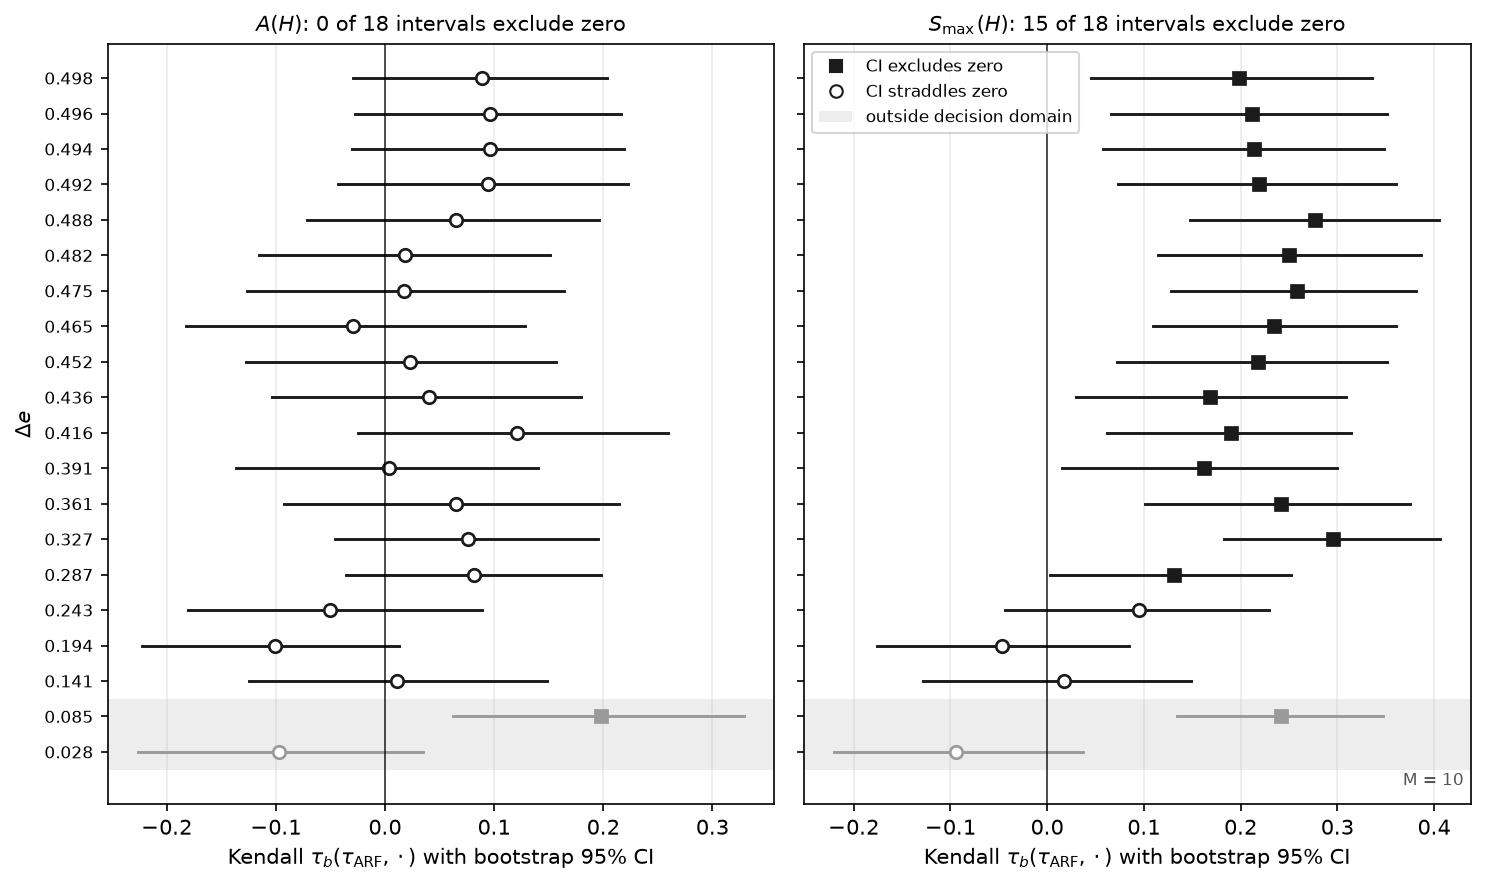
\includegraphics[width=\textwidth]{Fig_QD_forest_taub_full.png}
      \end{center}
    \end{column}
  \end{columns}
\end{frame}

% ==================================================================== 8
\begin{frame}{\fildariane{5}\hfill Détecter n'est pas gagner}
  \begin{columns}[c]
    \begin{column}{0.44\textwidth}
      \begin{center}
        \schemaZombie
      \end{center}
      \vspace{-0.4em}
      \begin{center}\tiny\color{gray}Schéma stylisé, sans données.\end{center}
    \end{column}
    \begin{column}{0.54\textwidth}
      \small
      À $\lambda = 15$ l'alarme part dans \textbf{$\num{92.9}$~\%} des exécutions
      --- mais elle n'arrive \emph{première} que dans \textbf{$\num{36.3}$~\%}.
      Le reste sonne après la réparation.

      \vspace{0.4em}
      Un taux de détection cité seul ne décrit donc pas le point aveugle.
    \end{column}
  \end{columns}

  \vspace{0.4em}
  \begin{center}
    \footnotesize
    \begin{tabular}{crrl}
      \toprule
      $\lambda$ & gagne la course & fausses alarmes & Wilson 95~\% \\
      \midrule
      $8$  & $\num{90.95}$~\% & $\num{4.15}$~\% & $[\num{3.36}\,;\,\num{5.12}]$ \\
      $10$ & $\num{89.95}$~\% & $\num{1.30}$~\% & $[\num{0.89}\,;\,\num{1.90}]$ \\
      $15$ & $\num{36.30}$~\% & $\num{0.15}$~\% & sous la résolution du témoin \\
      \bottomrule
    \end{tabular}
  \end{center}
  \vspace{-0.1em}
  {\scriptsize\color{gray}Témoin sans dérive porté à $\num{2000}$ exécutions le
  14/09 ; le rapport porte encore l'ancien, à $100$.}
\end{frame}

% ==================================================================== 9
\begin{frame}{\fildariane{5}\hfill Alors un seuil bas suffit-il ?}
  \begin{columns}[c]
    \begin{column}{0.47\textwidth}
      \begin{center}
        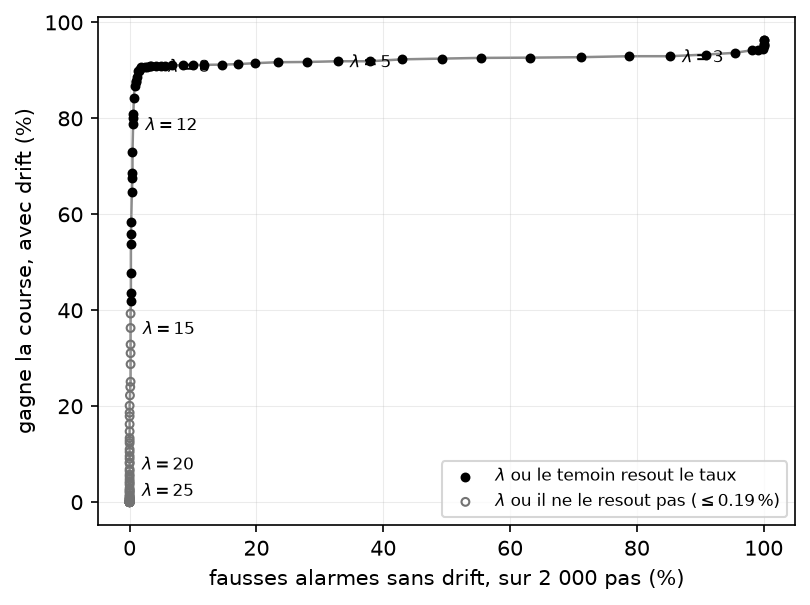
\includegraphics[height=0.53\textheight]{Fig_QE_compromis_lambda_n2000.png}
      \end{center}
    \end{column}
    \begin{column}{0.51\textwidth}
      \footnotesize
      Le coude est net, et c'est \textbf{gênant} : lu vite, ce graphique dit
      qu'un seuil autour de $\lambda = 10$ règle le problème pour presque rien.
      Sur notre banc, c'est exact.

      \vspace{0.4em}
      \textbf{Ce qui résiste quand même.} À $\Delta e = \num{0.028}$, \textbf{aucun}
      seuil admissible ne gagne une seule exécution sur cent. Le point aveugle
      des faibles amplitudes ne se règle par aucun réglage.

      \vspace{0.4em}
      \textbf{Trois réserves.} Banc de Bernoulli homoscédastique, donc rien sur
      les flux à volatilité groupée de l'article ; taux compté \emph{par
      exécution} de $\num{2000}$ pas, pas en temps moyen avant fausse alarme ;
      témoin aveugle sous $\num{0.19}$~\%.
    \end{column}
  \end{columns}

  \vspace{-0.4em}
  \question{Notre lecture --- « détecter n'est pas gagner, et sur ce banc
  l'ensemble admissible n'est pas vide » --- restreint le « aucun seuil n'y
  échappe » de l'article aux réglages qu'il a testés. On l'assume comme une
  correction, ou on la signale comme une limite de notre banc ?}
\end{frame}

% ==================================================================== 10
\begin{frame}{\fildariane{4}\hfill Piste --- la fenêtre de $A$}
  \vspace{-0.3em}
  \begin{center}
    \scalebox{0.74}{\schemaAire}
  \end{center}
  \vspace{-0.8em}
  \begin{center}\tiny\color{gray}Schéma stylisé, sans données.\end{center}

  \vspace{-0.1em}
  \footnotesize
  À forte amplitude la tâche d'après la rupture est plus \emph{facile} que
  l'ancienne : l'erreur passe sous son propre socle sur $\num{1934}$ des $\num{2000}$
  pas, et $A(H)$ \textbf{devient négative} dès $\Delta e = \num{0.482}$, jusqu'à
  $-\num{20.8}$. Le verdict « le chronomètre ne dit rien des dégâts » porte sur
  cette grandeur-là.

  \vspace{-0.2em}
  \question{Faut-il mesurer les dégâts sur la seule fenêtre de la transition
  plutôt que sur l'horizon entier --- et avec quelle règle de fenêtre, sachant
  que l'ajustement de l'article ne tient pas aux faibles amplitudes ? Le calcul
  se refait hors ligne, sans relancer de campagne.}
\end{frame}

% ==================================================================== 11
\begin{frame}{Les autres pistes --- toutes gratuites en calcul}
  \small
  \begin{itemize}
    \item \textbf{Le couple $(\lambda, \Delta e)$ plutôt que $\lambda$ seul.}
      La course se joue sur les deux : cartographier finement la transition,
      ou chercher un seuil qui s'adapte à l'amplitude.
    \item \textbf{Remplacer le chronomètre.} $\tau_{\mathrm{swap}}(50\%)$ est le
      meilleur compromis qu'on ait trouvé entre dégâts et alarme --- mais
      \emph{aucun} candidat ne passe encore le témoin sans dérive, qui est le
      contrôle éliminatoire.
    \item \textbf{Chiffrer le biais d'indépendance} au lieu d'en donner le
      signe, par un estimateur intra-exécution de la variance du terme commun.
    \item \textbf{L'erreur monte encore quand le premier arbre tombe}, sur cinq
      amplitudes. Ce n'est pas un artefact d'estimation : on ne sait pas
      l'expliquer.
    \item \textbf{Aucun résultat en fonction de $M$} : toute la campagne est à
      dix arbres. Les traces à d'autres tailles existent, sans trace de preuve.
  \end{itemize}

  \vspace{0.2em}
  {\footnotesize\color{gray}Toutes se calculent sur les tables déjà sur disque.
  Le balayage du seuil et la fenêtre de $A$ sont en revanche
  \textbf{exploratoires} : critères fixés après avoir vu les données, sans
  correction de multiplicité --- et ça se dira dans le rapport.}
\end{frame}

% ==================================================================== 12
\begin{frame}{Ce qu'on vous demande}
  \begin{columns}[t]
    \begin{column}{0.49\textwidth}
      \begin{block}{\small Sur le fond}
        \small
        \begin{enumerate}
          \item La portée de notre résultat sur le seuil (slide 9).
          \item La fenêtre sur laquelle mesurer les dégâts (slide 10).
          \item Parmi les pistes de la slide 11, laquelle vaut les jours qui
            restent ?
          \item \textbf{Ou bien autre chose :} y a-t-il une direction hors du
            sujet initial que vous aimeriez nous voir explorer ?
        \end{enumerate}
      \end{block}
    \end{column}
    \begin{column}{0.49\textwidth}
      \begin{block}{\small Sur la forme du rendu}
        \small
        \begin{enumerate}
          \item Les quinze pages sont-elles « tout compris » ? Une annexe
            est-elle admise en plus ?
          \item La déclaration d'usage des LLM compte-t-elle dans les pages ?
          \item \textbf{La date.} Les consignes annoncent « mardi
            16~septembre~» --- or le 16 est un mercredi. Laquelle des deux
            fait foi ?
        \end{enumerate}
      \end{block}
    \end{column}
  \end{columns}

  \vspace{0.6em}
  \begin{center}
    \small
    Et une question de Melaine : la séance facultative sur la thèse.
  \end{center}
\end{frame}

\end{document}
